%
\begin{isabellebody}%
\setisabellecontext{thesis{\isacharunderscore}{\isadigit{3}}{\isacharunderscore}implementation}%
%
\isadelimtheory
%
\endisadelimtheory
%
\isatagtheory
%
\endisatagtheory
{\isafoldtheory}%
%
\isadelimtheory
%
\endisadelimtheory
%
\isadelimdocument
%
\endisadelimdocument
%
\isatagdocument
%
\isamarkupsection{Implementation Details\label{details}%
}
\isamarkuptrue%
%
\endisatagdocument
{\isafolddocument}%
%
\isadelimdocument
%
\endisadelimdocument
%
\begin{isamarkuptext}%
In this section, I present the details of my implementation of automated Kantian ethics, which consists of
a formalization of the Formula of Universal Law in Dyadic Deontic Logic and an implementation of this logic in Isabelle/HOL. The final
Isabelle library contains a logic that has the categorical imperative as an axiom and can express and derive moral judgements. 
Using Isabelle's automated theorem proving abilities, my system can show that appropriately represented
maxims are obligatory, permissible, or prohibited by proving or refuting sentences of the form ``A 
is obligated to do B.'' I also present a testing framework to evaluate how faithful my implementation is 
to philosophical literature. This testing framework shows that my system outperforms unmodified DDL 
(a control group) and Moshe Kroy's prior formalization of the FUL \citep{kroy}.%
\end{isamarkuptext}\isamarkuptrue%
%
\isadelimdocument
%
\endisadelimdocument
%
\isatagdocument
%
\isamarkupsubsection{Formalization and Implementation of the FUL \label{implementation31}%
}
\isamarkuptrue%
%
\endisatagdocument
{\isafolddocument}%
%
\isadelimdocument
%
\endisadelimdocument
%
\begin{isamarkuptext}%
Formalizing the FUL requires implementing enough logical background to represent 
the FUL as an axiom. Dyadic Deontic Logic can express obligation and prohibition, but it cannot 
represent more complex features of moral judgement like actions, subject, maxims, and ends. I augment 
DDL by adding representations of these concepts, drawn from philosophical literature.%
\end{isamarkuptext}\isamarkuptrue%
%
\isadelimdocument
%
\endisadelimdocument
%
\isatagdocument
%
\isamarkupsubsubsection{Logical Background%
}
\isamarkuptrue%
%
\endisatagdocument
{\isafolddocument}%
%
\isadelimdocument
%
\endisadelimdocument
%
\begin{isamarkuptext}%
Kantian ethics is action-guiding; the categorical
imperative is a moral rule that agents can use to decide between potential actions. Thus, before I 
begin to formalize a specific formulation of the categorical imperative, I must define
subjects and act. I add representations of subjects and acts so that my new logic can express
sentences of the form, ``x does act.''%
\end{isamarkuptext}\isamarkuptrue%
\isacommand{typedecl}\isamarkupfalse%
\ s\ %
\isamarkupcmt{The new type $s$ is the type for a ``subject,'' as in the subject of a sentence.%
}%
\begin{isamarkuptext}%
The \texttt{typedecl} keyword indicates that I am defining a new atomic type, which is not composed
of pre-existing types but is instead a new kind of object altogether. A type does not come with any 
properties out of the box. There is no difference between declaring a type with label ``subject'' or any other
label, such as ``color'' or ``mammal.'' I add some properties of this type below by creating formulas
and more complex types that use this type, but I do not provide a complete definition of a subject.
Formalizing and using the FUL does not require many of the complex properties of a subject, such as 
rationality or humanity. Thus, instead of providing a complete definition of subject, I can avoid murky
philosophical debates about the nature of agency and instead provide a 
``thin'' definition that only includes the minimum necessary properties to apply the FUL. Throughout my 
project, I will use bare syntactic units like types and constants to create thin definitions of new ideas.
This strategy lets me avoid messy philosophical controversies and makes my system's judgements more 
trustworthy, because they rely on relatively little prior knowledge.

In this interpretation, the defining feature of a subject is that they can act. 
I represent that below by allowing subjects to substitute into sentences, a property that I will use 
to represent the idea that different people can perform the same acts.%
\end{isamarkuptext}\isamarkuptrue%
\isacommand{type{\isacharunderscore}synonym}\isamarkupfalse%
\ os\ {\isacharequal}\ {\isachardoublequoteopen}{\isacharparenleft}s\ {\isasymRightarrow}\ t{\isacharparenright}{\isachardoublequoteclose}\ \isanewline
%
\isamarkupcmt{To model the idea of a subject being substituted into an action, I 
define \texttt{type\_synonym} $os$ for an open sentence. An open sentence takes as input a subject and 
returns a complete or ``closed'' DDL formula by binding the free variable in the sentence to the input. 
For example, ``runs'' is an open sentence that can be instantiated with subject, ``Sara'' to create
the DDL term ``Sara runs,'' which can be true or false at a world. An open sentence itself is not truth-apt,
ot the kind of thing that can be true or false at a world. When a subject is 
substituted into an open sentence, the resulting term is truth apt. ``Runs'' is not the kind of thing 
that can be true or false, but ``Sara runs'' is a sentence that can be true or false.%
}%
\isadelimdocument
%
\endisadelimdocument
%
\isatagdocument
%
\isamarkupsubsubsection{Maxims \label{whatisamaxim}%
}
\isamarkuptrue%
%
\endisatagdocument
{\isafolddocument}%
%
\isadelimdocument
%
\endisadelimdocument
%
\begin{isamarkuptext}%
As established in Section \ref{whyful}, I formalize a version of the categorical imperative called
the Formula of Universal, which reads ``act only according to that maxim by which you can at the same 
time will that it should become a universal law'' \citep[34]{groundwork}. In order to faithfully formalize
the FUL, I must make precise what it means to will a maxim and what kinds of maxims can become universal laws. 
I draw on reliable definitions of willing, maxims, and universalization from Kantian literature and represent them in DDL.
Throughout this section, I will use one of Kant's canonical maxims as an example.

\begin{example}[False Promising]\label{falsepromise}
  The false promising example maxim reads, ``When I am strapped for cash, I will falsely promise to repay a loan 
to get some easy cash.''
\end{example}

The central unit of evaluation for Kantian ethics is a ``maxim,'' which Kant defines as ``the subjective 
principle of willing,'' or the principle that the agent understands themselves as acting on \citep[16, footnote 1]{groundwork}. 
Modern Kantians differ in their interpretations of this definition. I adopt O'Neill's view, derived from 
Kant's example maxims, that a maxim includes the act, the circumstances, and the agent's purpose of 
acting or goal \citep{actingonprinciple}. Other potential views include Korsgaard's view, which omits 
the circumstances, and Kitcher's view, which additionally includes the actor's motivation \citep{actingforareason, kitcher}. I 
address the limitations of these approaches in Appendix \ref{maximmotive}.


\begin{definition}[Maxim]
    A maxim is a circumstance, act, goal tuple (C, A, G), read as ``In circumstances C, act A for goal G.''
\end{definition}

I implement this definition in Isabelle by defining the \texttt{type\_synonym} below for the type
of a maxim.%
\end{isamarkuptext}\isamarkuptrue%
\isacommand{type{\isacharunderscore}synonym}\isamarkupfalse%
\ maxim\ {\isacharequal}\ {\isachardoublequoteopen}{\isacharparenleft}t\ {\isacharasterisk}\ os\ {\isacharasterisk}\ t{\isacharparenright}{\isachardoublequoteclose}\isanewline
%
\isamarkupcmt{A maxim is of type term, open sentence, term tuple, such as ``(When I am strapped for cash, will falsely promise
to repay a loan, to get some easy cash)''. The first term represents the circumstance, which
can be true or false at a world. For example, the circumstance ``when I am strapped for cash'' is true at the real 
world when my bank account is empty. The second term represents the act, which is an open sentence
because different agents can perform a particular action. For example, the act, ``will falsely promise
to repay a loan'' is an open sentence that can be acted on by a subject. The third term represents 
the goal, which can again be true or false at a world. For example, the goal ``to get some easy cash''
is true at the real world if I have successfully received easy cash.%
}%
\begin{isamarkuptext}%
O'Neill argues that a maxim 
is an action-guiding rule and thus naturally includes an act and the circumstances under which 
it should be performed \citep[37]{actingonprinciple}. 
She also includes a purpose, end, or goal in the maxim because human activity is guided by a rational will
and is thus inherently purposive \citep[40]{groundwork}. A rational will does not act randomly (else it would not be rational), 
but instead in the pursuit of ends which it deems valuable. The inclusion a maxim's end is essential 
for the version of the FUL that I will implement, explained in Section \ref{praccon}.

O'Neill's inclusion of circumstances is potentially controversial because it leaves open the question of what qualifies as a 
relevant circumstance for a particular maxim. This gives rise to ``the tailoring objection,'' 
under which maxims are arbitrarily specified to pass the FUL  \citep[217]{whatisamaxim}. \footnote{Kitcher
cites \citet{kantsethicalthought} as offering an example of a false positive due to this objection.} For example, the maxim ``When my name is Jane Doe
and I am wearing a purple shirt and it is Tuesday morning, I will murder my boss so I can take their job,'' 
is universalizable but is clearly a false positive because we think that murder for professional gain is wrong. 
One solution to this problem is to argue that the circumstance ``When my name is Jane Doe and I am wearing a 
purple shirt and it is Tuesday morning'' is not morally relevant 
to the act and goal. This solution requires determining what qualifies as a relevant circumstance.

O'Neill seems to acknowledge the difficulty of determining relevant circumstances when she concedes that a maxim cannot include all 
of the infinitely many circumstances in which the agent may perform an action \citep[4:428]{actingonprinciple}. She argues that this is 
an artifact of the fact that maxims are rules of practical reason, which is the kind of reason that helps us decide what to do 
and how to do it \citep{bok}. Like any practical rule, 
maxims require the exercise of practical judgement to determine in which circumstances they should be applied. 
This judgement, applied in both choosing when to exercise the maxim and in the formulation of the maxim 
itself, is what determines the morally relevant circumstances.  
The difficulty in determining relevant circumstances is an obstacle to using my system in practice and requires that a 
human being formulate the maxim or that future work develop heuristics to classify circumstances as morally 
relevant. I discuss this challenge and potential solutions in greater detail in Section \ref{AIethics}.

With this robust representation of a maxim, I can now define willing. To will a maxim is to adopt it 
as a principle to live by, or to commit oneself to the maxim's act for the 
sake of maxim's end in the relevant circumstances. I formalize this idea in Definition \ref{willing}.

\begin{definition}[Willing]\label{willing}
For maxim $M = (C, A, G)$ and actor $s$,
$$\text{\emph{will}} \, M \, s \equiv \forall w \, (C \longrightarrow A \, (s)) \, w$$
\noindent At all worlds $w$, if the circumstances hold at that world, agent $s$ performs act $A$.
\end{definition}

If I will the example \nameref{falsepromise} maxim, then whenever I need cash, 
I will falsely promise to repay a loan. I can represent this definition using the following Isabelle
formula.%
\end{isamarkuptext}\isamarkuptrue%
\isacommand{abbreviation}\isamarkupfalse%
\ will\ {\isacharcolon}{\isacharcolon}\ {\isachardoublequoteopen}maxim\ {\isasymRightarrow}\ s{\isasymRightarrow}\ \ t{\isachardoublequoteclose}\ {\isacharparenleft}{\isachardoublequoteopen}W\ {\isacharunderscore}\ {\isacharunderscore}{\isachardoublequoteclose}{\isacharparenright}\isanewline
\ \ \isakeyword{where}\ {\isachardoublequoteopen}will\ {\isasymequiv}\ {\isasymlambda}{\isacharparenleft}c{\isacharcomma}\ a{\isacharcomma}\ g{\isacharparenright}\ s{\isachardot}\ {\isacharparenleft}c\ \isactrlbold {\isasymrightarrow}\ {\isacharparenleft}a\ s{\isacharparenright}{\isacharparenright}{\isachardoublequoteclose}\isanewline
%
\isamarkupcmt{An agent $s$ wills a maxim if in the circumstances, $s$ performs the action, or $s$ substituted
into the open sentence $a$ is true. This is an Isabelle \texttt{abbreviation}, which is syntactic
sugar for an Isabelle formula. The type of this formula is $maxim \rightarrow s \rightarrow t$, so it 
takes as input a maxim and a subject and returns the term, ``s wills maxim.''%
}%
\isadelimdocument
%
\endisadelimdocument
%
\isatagdocument
%
\isamarkupsubsubsection{Practical Contradiction Interpretation of the FUL \label{praccon}%
}
\isamarkuptrue%
%
\endisatagdocument
{\isafolddocument}%
%
\isadelimdocument
%
\endisadelimdocument
%
\begin{isamarkuptext}%
In order to evaluate the moral status of a maxim, I must define what it means for a maxim to not be
universalizable, or to fail the universalizability test. For many years, Kantians debated the correct interpretation of 
the Formula of Universal Law because Kant himself appeared to interpret the criterion in different ways. 
I adopt Korsgaard's practical contradiction interpretation, broadly accepted as correct within 
the philosophical community \citep{ebelsduggan}.
 
Recall that the Formula of Universal Law is to “act only in accordance with that maxim through which 
you can at the same time will that it become a universal law” \citep[34]{groundwork}. To determine if a 
maxim can be willed as a universal law, we use the “universalizability test,” which requires 
imagining a world in which everyone has willed the maxim. If willing the maxim in such a world 
generates a contradiction, then the action is prohibited. For example, the \nameref{falsepromise}
maxim will be prohibited if it is impossible to will the maxim in a world where everyone falsely promises
to repay loans.

One interpretation of the FUL, the logical contradiction interpretation, prohibits maxims that are 
logically impossible when universalized. Under this view, falsely promising to repay a loan fails the 
universalizability test because, in the universalized world, everyone falsely promises to repay
loans so lenders no longer believe promises to repay loans. The practice of giving loans would die out, so 
making a false promise to repay a loan would be impossible.

This view cannot correctly handle natural acts. Korsgaard appeals to 
\citet{dietrichson} to construct the example natural act of a mother killing her children that
cry too much at night so that she can get some sleep. Thought this maxim is clearly wrong, universalizing 
it does not generate a logical contradiction because killing is still possible in a world where 
everyone kills noisy children. Because killing is a natural act, it can never be logically 
impossible so the logical contradiction view cannot prohibit it.

As an alternative to the logical contradiction view, Korsgaard endorses the practical contradiction view, 
which prohibits maxims that are self-defeating, or ineffective, when universalized. By willing a maxim, 
you commit yourself to the maxim's goal, and thus cannot rationally will that this goal be 
undercut. This interpretation can prohibit natural acts like those of the sleep-deprived mother: in 
willing the end of sleeping, she is implicitly willing that she is alive. If all mothers kill all 
loud children, then she cannot be secure in the possession of her life, because her own mother may 
have killed her as an infant. Her willing this maxim thwarts the end that she sought to secure. 

The practical contradiction interpretation offers a satisfying explanation of \emph{why} certain 
maxims are immoral. These maxims involve parasitic behavior on the very social conditions that the agent seeks 
to benefit from. The false promiser wants to both abuse the system of promising and benefit 
from it, and is thus making an exception of themselves. The test formalizes the kinds of objections 
that the question ``What if everyone did that?'' seeks to draw out.\footnote{This argument for the practical
contradiction interpretation is due to \citet{KorsgaardFUL}.}

Under the practical contradiction interpretation, the FUL states, ``If, when universalized, a maxim is 
not effective, then it is prohibited.'' This requires defining effectiveness and universalization. 
If an agent wills an effective maxim, then the maxim's goal is achieved, and if the agent does 
not will it, then the goal is not achieved. 

\begin{definition}[Effective Maxim]
For a maxim $M = (C, A, G)$ and actor $s$,
$$\text{\emph{effective}} \, M \, s \equiv \forall w \, (\text{\emph{will}} \, (C, A, G) \, s \iff G) \, w$$
\end{definition}
\noindent I implement this in Isabelle below.%
\end{isamarkuptext}\isamarkuptrue%
\isacommand{abbreviation}\isamarkupfalse%
\ effective\ {\isacharcolon}{\isacharcolon}\ {\isachardoublequoteopen}maxim{\isasymRightarrow}s{\isasymRightarrow}\ t{\isachardoublequoteclose}\ {\isacharparenleft}{\isachardoublequoteopen}E\ {\isacharunderscore}\ {\isacharunderscore}{\isachardoublequoteclose}{\isacharparenright}\isanewline
\ \ \isakeyword{where}\ {\isachardoublequoteopen}effective\ \ {\isasymequiv}\ {\isasymlambda}{\isacharparenleft}c{\isacharcomma}\ a{\isacharcomma}\ g{\isacharparenright}\ s{\isachardot}\ {\isacharparenleft}{\isacharparenleft}will\ {\isacharparenleft}c{\isacharcomma}\ a{\isacharcomma}\ g{\isacharparenright}\ s{\isacharparenright}\ \isactrlbold {\isasymequiv}\ g{\isacharparenright}{\isachardoublequoteclose}\isanewline
%
\isamarkupcmt{A maxim is effective for a subject if the goal is achieved if and only if the subject wills the maxim.
Once again, I use an abbreviation to conveniently refer to this Isabelle formula.%
}%
\begin{isamarkuptext}%
The former direction of the implication is intuitive: if the act results in the goal, it was 
effective in causing the goal. This represents sufficient causality. The latter direction represents 
necessary causality, or the idea that, counterfactually, if the maxim were not willed, then the goal 
would not be achieved \citep{lewiscausality}.\footnote{Thank you to Jeremy Zucker for helping me 
think about causality in this way.}
Combining these ideas, this definition of effective states that a maxim is effective if the 
maxim being acted on by a subject is the necessary and sufficient cause of the goal.

Next, I define what it means for a maxim to be universalized. Recall that the universalizability 
test requires imagining a world in which everyone wills a maxim. Therefore, a maxim is universalized
when everyone wills the maxim. 

\begin{definition}[Universalized]
  For a maxim $M$ and agent $s$,
$$\text{\emph{universalized}} \, M  \equiv \forall w \, (\forall p \, \text{\emph{will}} \, M \, p)$$
\end{definition}

\noindent I can once again represent this as an abbreviation in Isabelle.%
\end{isamarkuptext}\isamarkuptrue%
\isacommand{abbreviation}\isamarkupfalse%
\ universalized{\isacharcolon}{\isacharcolon}{\isachardoublequoteopen}maxim{\isasymRightarrow}t{\isachardoublequoteclose}\ \isakeyword{where}\ \isanewline
{\isachardoublequoteopen}universalized\ {\isasymequiv}\ {\isasymlambda}M{\isachardot}\ {\isacharparenleft}{\isasymlambda}w{\isachardot}\ {\isacharparenleft}{\isasymforall}p{\isachardot}\ {\isacharparenleft}W\ M\ p{\isacharparenright}\ w{\isacharparenright}{\isacharparenright}{\isachardoublequoteclose}\isanewline
%
\isamarkupcmt{The abbreviation $universalized$ takes a maxim as input and returns a term which is true at a world 
if all people at that world will the maxim.%
}%
\begin{isamarkuptext}%
With the above definitions of effective and universalization, I can define what it means for 
a maxim to not be universalizable. This is the core of the FUL, which states that if a maxim is not 
universalizable, it is prohibited. Under the practical contradiction interpretation, a maxim is 
not universalizable if, when universalized, it is no longer effective.

\begin{definition}[Not Universalizable]
For a maxim $M$ and agent $s$,
$$\text{\emph{not\_universalizable}} \, M \, s  \equiv [ \text{\emph{universalized}} \, M \longrightarrow \neg \, \text{\emph{effective}} \, M \, s ]$$
\end{definition}
\noindent A maxim is not universalizable when, if everyone wills the maxim, then it is no longer 
effective. I implement this definition in Isabelle using another abbreviaion.%
\end{isamarkuptext}\isamarkuptrue%
\isacommand{abbreviation}\isamarkupfalse%
\ not{\isacharunderscore}universalizable\ {\isacharcolon}{\isacharcolon}\ {\isachardoublequoteopen}maxim{\isasymRightarrow}s{\isasymRightarrow}bool{\isachardoublequoteclose}\ \isakeyword{where}\ \isanewline
{\isachardoublequoteopen}not{\isacharunderscore}universalizable\ {\isasymequiv}\ {\isasymlambda}M\ s{\isachardot}\ {\isasymforall}w{\isachardot}\ {\isacharparenleft}{\isacharparenleft}universalized\ M{\isacharparenright}\ \ \isactrlbold {\isasymrightarrow}\ {\isacharparenleft}\isactrlbold {\isasymnot}\ {\isacharparenleft}E\ M\ s{\isacharparenright}{\isacharparenright}{\isacharparenright}\ w{\isachardoublequoteclose}\isanewline
%
\isamarkupcmt{Maxim $M$ is not universalizable at world $w$ when, ``at world $w$, if M is universalized, then M is not effective.''%
}%
\begin{isamarkuptext}%
The FUL states that if a maxim is not universalizable, then it is prohibited. To define and use 
this statement, I must first define obligation, permissibility, and prohibition.
To judge a maxim, my system evaluates the moral status of the sentence 
``person $s$ wills maxim $M$.'' This action can be obligated, prohibited, or permissible.
I will use the phrase ``subject $s$ willing maxim $M$ is obligatory" 
interchangeably with ``maxim $M$ is obligatory for subject $s$." I will use ``maxim $M$ is obligatory" to 
refer to $M$ being obligatory for any arbitrary subject, which is equivalent to $M$ being 
obligatory for a specific subject.\footnote{The full proof for this result is the Obligation Universalizes
Across People Test in Section \ref{testing}.}

\begin{definition}[Obligation]

Let maxim $M$ be composed of the circumstances, act, goal tuple $C, A, G$ and let $s$ be an arbitrary agent.
$$\text{\emph{obligated}} \, M \, s \equiv O\{ \text{\emph{will}} \, (C, A, G) \, s \, | \, C\}$$
\end{definition}

The action ``$s$ wills $M$'' is the first argument passed to the dyadic obligation operator and is 
thus the action that is shown to be obligated or not. The second argument passed to the obligation 
operator represents the context in which the obligation holds and is thus naturally the maxim's circumstances.
This definition does not require any additional syntactic sugar, since it merely uses the dyadic obligation
operator. Using this definition, I can define prohibition and permissibility.

\begin{definition}[Prohibition and Permissibility] Let maxim $M$ be composed of the circumstances, act, 
goal tuple $C, A, G$ and let $s$ be an arbitrary agent.\footnote{Technically, a maxim is not a boolean 
type, so the term $\neg M$ is not type correct. The expression $obligated \, \neg M$ merely provides 
intuition for the meaning of prohibition, but the exact definition is given by 
$O\{ \neg \text{will} \, (C, A, G) \, s \, | \, C\}$.}
\newcommand*{\approxident}{%
  \mathrel{\vcenter{\offinterlineskip
  \hbox{$\sim$}\vskip-.35ex\hbox{$\sim$}\vskip-.35ex\hbox{$\sim$}}}}
$$\text{\emph{prohibited}} \, M \, s \approxident \text{\emph{obligated}} \, \neg M \, \equiv O\{ \neg \text{\emph{will}} \, (C, A, G) \, s \, | \, C\}$$
$$\text{\emph{permissible}} \, M \, s \equiv \neg \text{\emph{prohibited}} \, M \, s \equiv \neg O\{ \neg \text{\emph{will}} \, (C, A, G) \, s \, | \, C\}$$
\end{definition}%
\end{isamarkuptext}\isamarkuptrue%
\isacommand{abbreviation}\isamarkupfalse%
\ prohibited{\isacharcolon}{\isacharcolon}{\isachardoublequoteopen}maxim{\isasymRightarrow}s{\isasymRightarrow}t{\isachardoublequoteclose}\ \isakeyword{where}\ \isanewline
{\isachardoublequoteopen}prohibited\ {\isasymequiv}\ {\isasymlambda}{\isacharparenleft}c{\isacharcomma}\ a{\isacharcomma}\ g{\isacharparenright}\ s{\isachardot}\ O{\isacharbraceleft}\isactrlbold {\isasymnot}\ {\isacharparenleft}will\ {\isacharparenleft}c{\isacharcomma}a{\isacharcomma}\ g{\isacharparenright}\ s{\isacharparenright}\ {\isacharbar}\ c{\isacharbraceright}{\isachardoublequoteclose}\isanewline
%
\isamarkupcmt{A maxim is prohibited for a subject $s$ if its negation is obligated for $s$. It is morally wrong 
for an agent to will a prohibited maxim.%
}\isanewline
\isacommand{abbreviation}\isamarkupfalse%
\ permissible{\isacharcolon}{\isacharcolon}{\isachardoublequoteopen}maxim{\isasymRightarrow}s{\isasymRightarrow}t{\isachardoublequoteclose}\isanewline
\ \ \isakeyword{where}\ {\isachardoublequoteopen}permissible\ {\isasymequiv}\ {\isasymlambda}M\ s{\isachardot}\ \isactrlbold {\isasymnot}\ {\isacharparenleft}prohibited\ M\ s{\isacharparenright}{\isachardoublequoteclose}\isanewline
%
\isamarkupcmt{A maxim is permissible for a subject $s$ if it is not prohibited for $s$. It is morally acceptable 
for an agent to will or not will a permissible maxim.%
}%
\begin{isamarkuptext}%
One additional piece of logical background necessary before I implement the FUL is the 
notion of contradictory obligations. Many deontic logics, including DDL, allow contradictory
obligations. As I will explain in Section \ref{testing}, Kantian ethics never prescribes contradictory
obligations, so I will add this as an axiom.%
\end{isamarkuptext}\isamarkuptrue%
\isacommand{abbreviation}\isamarkupfalse%
\ non{\isacharunderscore}contradictory\ \isakeyword{where}\ \isanewline
{\isachardoublequoteopen}non{\isacharunderscore}contradictory\ A\ B\ c\ w\ {\isasymequiv}\ {\isacharparenleft}{\isacharparenleft}O{\isacharbraceleft}A{\isacharbar}c{\isacharbraceright}\ \isactrlbold {\isasymand}\ O{\isacharbraceleft}B{\isacharbar}c{\isacharbraceright}{\isacharparenright}\ w{\isacharparenright}\ {\isasymlongrightarrow}\ {\isasymnot}{\isacharparenleft}{\isacharparenleft}A\ \isactrlbold {\isasymand}\ {\isacharparenleft}B\ \isactrlbold {\isasymand}\ c{\isacharparenright}{\isacharparenright}\ w\ {\isasymlongrightarrow}\ False{\isacharparenright}{\isachardoublequoteclose}\isanewline
%
\isamarkupcmt{Terms $A$ and $B$ are non contradictory in circumstances $c$ if, when $A$ and $B$ are obligated in circumstances 
$c$, the conjunction of $A$, $B$, and $c$, does not imply $False$.%
}\isanewline
\isacommand{axiomatization}\isamarkupfalse%
\ \isakeyword{where}\ no{\isacharunderscore}contradictions{\isacharcolon}{\isachardoublequoteopen}{\isasymforall}A{\isacharcolon}{\isacharcolon}t{\isachardot}\ {\isasymforall}B{\isacharcolon}{\isacharcolon}t{\isachardot}\ {\isasymforall}c{\isacharcolon}{\isacharcolon}t{\isachardot}\ {\isasymforall}w{\isacharcolon}{\isacharcolon}i{\isachardot}\ non{\isacharunderscore}contradictory\ A\ B\ c\ w{\isachardoublequoteclose}\isanewline
%
\isamarkupcmt{This axiom formalizes the idea that, for any terms $A$, $B$, and circumstances $c$, $A$, and $B$ must be 
non-contradictory in circumstances $c$ at all worlds. Intuitively, this axiom requires that obligations 
do not conflict.%
}%
\isadelimdocument
%
\endisadelimdocument
%
\isatagdocument
%
\isamarkupsubsubsection{Formalizing the FUL\label{formalizingful}%
}
\isamarkuptrue%
%
\endisatagdocument
{\isafolddocument}%
%
\isadelimdocument
%
\endisadelimdocument
%
\begin{isamarkuptext}%
With this logical background, I can begin to implement the Formula of Universal Law, which, as defined 
by the practical contradiction interpretation, states that a maxim is prohibited if it is ineffective
when universalized. A first, unsuccessful attempt to formalize the FUL simply translates this into Isabelle's syntax
using the abbreviations above. While this attempt will not be consistent, I will use Isabelle's automatic
proof search abilities to determine how to modify this formula to be consistent, revealing a key philosophical
insight about maxims in the process. This section presents my final formalization of the FUL and the 
philosophical insight produced while creating it, which, as I argue in Section \ref{computationalethics},
demonstrates the power of computational tools in aiding philosophical progress.%
\end{isamarkuptext}\isamarkuptrue%
\isacommand{abbreviation}\isamarkupfalse%
\ FUL{\isadigit{0}}{\isacharcolon}{\isacharcolon}bool\ \isakeyword{where}\ {\isachardoublequoteopen}FUL{\isadigit{0}}\ {\isasymequiv}\ {\isasymforall}\ c\ a\ g\ s{\isachardot}\ not{\isacharunderscore}universalizable\ {\isacharparenleft}c{\isacharcomma}\ a{\isacharcomma}\ g{\isacharparenright}\ s\ {\isasymlongrightarrow}\ {\isasymTurnstile}{\isacharparenleft}{\isacharparenleft}prohibited\ {\isacharparenleft}c{\isacharcomma}\ a{\isacharcomma}\ g{\isacharparenright}\ s{\isacharparenright}{\isacharparenright}{\isachardoublequoteclose}\isanewline
%
\isamarkupcmt{This representation of the Formula of Universal Law reads, ``For all circumstances, goals, acts, 
and subjects, if the maxim of the subject performing the act for the goal in the circumstances is not 
universalizable (as defined above), then, at all worlds, in those circumstances, the subject 
is prohibited from (obligated not to) willing the maxim.''%
}%
\begin{isamarkuptext}%
I can immediately determine if this version of the FUL is consistent by checking if \texttt{FUL0} 
implies $False$.%
\end{isamarkuptext}\isamarkuptrue%
\isacommand{lemma}\isamarkupfalse%
\ {\isachardoublequoteopen}FUL{\isadigit{0}}\ {\isasymlongrightarrow}\ False{\isachardoublequoteclose}%
\isadelimproof
\ %
\endisadelimproof
%
\isatagproof
\isacommand{using}\isamarkupfalse%
\ O{\isacharunderscore}diamond\isanewline
\ \ \isacommand{using}\isamarkupfalse%
\ case{\isacharunderscore}prod{\isacharunderscore}conv\ no{\isacharunderscore}contradictions\ old{\isachardot}prod{\isachardot}case\ old{\isachardot}prod{\isachardot}case\ \isacommand{by}\isamarkupfalse%
\ fastforce%
\endisatagproof
{\isafoldproof}%
%
\isadelimproof
%
\endisadelimproof
%
\begin{isamarkuptext}%
Isabelle's proof-finding tool, Sledgehammer, shows that 
\texttt{FUL0} is not consistent by showing that it implies a contradiction 
using axiom \texttt{O\_diamond}\footnote{The full axiom reads \isa{{\isasymTurnstile}{\isasymlambda}w{\isachardot}\ ob\ {\isacharquery}B\ {\isacharquery}A\ {\isasymlongrightarrow}\ {\isasymnot}\ {\isasymTurnstile}\isactrlbold {\isasymnot}\ {\isacharquery}B\isactrlbold {\isasymand}{\isacharquery}A}.} \citep{sledgehammer}. 
This axiom roughly states that an obligation can't contradict its context. Knowing that \texttt{FUL0}
contradicts this particular axiom offers insight into what the problem is. If the goal or action
or a maxim are equivalent to its circumstance, then prohibiting it is contradictory. If the maxim has already been 
acted on or the goal has already been achieved, then the agent cannot undo their action or the achivement 
of the goal. 

This motivates the exclusion of what I call ``badly formed maxims,'' which are those maxims such that 
the goal has already been achieved or the act has already been acted on. Under my formalization, such maxims are
not well-formed. 

\begin{definition}[Well-Formed Maxim]
A maxim is well-formed if the circumstances do not contain the act and goal. For a maxim $(C, A, G)$, and subject $s$, 
$$ \text{\emph{well\_formed}} \, (C, A, G) \, s \equiv \forall w \, (\neg (C \longrightarrow G) \wedge \neg (C \longrightarrow A \, s)) \, w$$

\end{definition}

For example, the maxim ``When I eat breakfast, I will eat breakfast to eat breakfast'' is badly-formed
because the circumstance ``when I eat breakfast'' contains the act and goal. Well-formedness is not 
discussed in the literature, but I find that if I require that the FUL only holds for well-formed maxim, it is
consistent.%
\end{isamarkuptext}\isamarkuptrue%
\isacommand{abbreviation}\isamarkupfalse%
\ well{\isacharunderscore}formed{\isacharcolon}{\isacharcolon}{\isachardoublequoteopen}maxim{\isasymRightarrow}s{\isasymRightarrow}i{\isasymRightarrow}bool{\isachardoublequoteclose}\ \isakeyword{where}\ \isanewline
{\isachardoublequoteopen}well{\isacharunderscore}formed\ {\isasymequiv}\ {\isasymlambda}{\isacharparenleft}c{\isacharcomma}\ a{\isacharcomma}\ g{\isacharparenright}{\isachardot}\ {\isasymlambda}s{\isachardot}\ {\isasymlambda}w{\isachardot}\ {\isacharparenleft}{\isasymnot}\ \ {\isacharparenleft}c\ \isactrlbold {\isasymrightarrow}\ g{\isacharparenright}\ w{\isacharparenright}\ {\isasymand}\ {\isacharparenleft}{\isasymnot}\ \ {\isacharparenleft}c\ \isactrlbold {\isasymrightarrow}\ a\ s{\isacharparenright}\ w{\isacharparenright}{\isachardoublequoteclose}\isanewline
%
\isamarkupcmt{This abbreviation formalizes the well-formedness of a maxim for a subject. The goal cannot be 
already achieved in the circumstances and the subject cannot have already performed the act.%
}%
\begin{isamarkuptext}%
\noindent If I modify \texttt{FUL0} to only hold for well-formed maxims, it becomes consistent.%
\end{isamarkuptext}\isamarkuptrue%
\isacommand{abbreviation}\isamarkupfalse%
\ FUL\ \isakeyword{where}\ \isanewline
{\isachardoublequoteopen}FUL\ {\isasymequiv}\ {\isasymforall}M{\isacharcolon}{\isacharcolon}maxim{\isachardot}\ {\isasymforall}s{\isacharcolon}{\isacharcolon}s{\isachardot}\ {\isacharparenleft}{\isasymforall}w{\isachardot}\ well{\isacharunderscore}formed\ M\ s\ w{\isacharparenright}\ {\isasymlongrightarrow}\ {\isacharparenleft}not{\isacharunderscore}universalizable\ M\ s\ {\isasymlongrightarrow}\ {\isasymTurnstile}\ {\isacharparenleft}prohibited\ M\ s{\isacharparenright}\ {\isacharparenright}{\isachardoublequoteclose}\isanewline
%
\isamarkupcmt{This formalization states that if a maxim is well-formed, then if it is not universalizable, 
it is prohibited.%
}\isanewline
\isanewline
\isacommand{lemma}\isamarkupfalse%
\ {\isachardoublequoteopen}FUL{\isachardoublequoteclose}\isanewline
\ \ \isacommand{nitpick}\isamarkupfalse%
{\isacharbrackleft}user{\isacharunderscore}axioms{\isacharcomma}\ falsify{\isacharequal}false{\isacharbrackright}%
\isadelimproof
\ %
\endisadelimproof
%
\isatagproof
\isacommand{oops}\isamarkupfalse%
\isanewline
%
\isamarkupcmt{Nitpick is Isabelle's countermodel checker, and I can use it to quickly check that an axiom is 
consistent \citep{nitpick}. If Nitpick can find a model in which the axioms of DDL hold and the FUL is 
true, then it is consistent.

\color{blue} Nitpick found a model for card $i$ = 1 and card $s$ = 2:

  Empty assignment \color{black}%
}%
\endisatagproof
{\isafoldproof}%
%
\isadelimproof
%
\endisadelimproof
%
\begin{isamarkuptext}%
My above investigation of \texttt{FUL0} shows that if the FUL holds for badly formed maxims, then 
it is inconsistent. This is not only a logical property of my system, but it also has philosophical
significance that coheres with Korsgaard's and O'Neill's interpretations of a maxim as a practical
guide to action \citep{actingforareason,actingonprinciple}. A maxim is a practical principle that guides how we behave in everyday life. A 
principle of the form ``When you are eating breakfast, eat breakfast in order to eat breakfast,'' is not 
practically relevant. No agent would ever need to act on such a principle. Morality helps agents decide
whether to act on a potential principle of action, but no agent would need to ask
``When I am eating breakfast, should I eat breakfast in order to eat breakfast?" It is the wrong kind of 
principle to be evaluating. It is not a well-formed maxim, so the categorical imperative cannot apply to it. 

The fact that Isabelle revealed a philosophical insight about which kinds of maxims are well-formed
is an example of the power of computational tools to aid
philosophical progress. Nitpick and Sledgehammer helped me confirm that certain kinds
of circumstance, act, goal tuples are too badly formed for the categorical imperative to logically 
apply to them. The realization of this subtle problem would have been incredibly difficult without 
computational tools, and serves as evidence of the power of computational ethics. I discuss the philosophical
properties and implications of well-formed maxims and the power of computational ethics further in 
Section \ref{computationalethics}.

I complete my implementation by adding the consistent version of the FUL as an axiom.%
\end{isamarkuptext}\isamarkuptrue%
\isacommand{axiomatization}\isamarkupfalse%
\ \isakeyword{where}\ FUL{\isacharcolon}FUL%
\begin{isamarkuptext}%
This concludes my implementation of the Formula of Universal Law in Isabelle/HOL. My implementation
consistents of necessary logical background, first formalized in DDL and then implemented in Isabelle.
The code snippets in this chapter are a subset of over 100 lines of Isabelle/HOL code necessary to
complete this implementation. In Section \ref{testing} and Chapter \ref{applications}, I demonstrate how this
implementation can be tested and used to make moral judgements.%
\end{isamarkuptext}\isamarkuptrue%
%
\isadelimdocument
%
\endisadelimdocument
%
\isatagdocument
%
\isamarkupsubsection{Tests\label{testing}%
}
\isamarkuptrue%
%
\endisatagdocument
{\isafolddocument}%
%
\isadelimdocument
%
\endisadelimdocument
%
\begin{isamarkuptext}%
In addition to an implementation of automated Kantian ethics, I also contribute a testing framework 
to evaluate how well my implementation coheres with philosophical literature. This testing architecture 
makes the notion of ``philosophical faithfulness'' precise. Each test consists of a sentence in my logic 
and an expected outcome, where the possible outcomes are proving or refuting the sentence. For example, 
one such sentence is that obligations cannot contradict each other. To run the tests, I attempt to
 prove or refute each test sentence in my logic.  Because these tests are derived from moral 
intuition and philosophical literature, they evaluate how well my system reflects philosophical
literature. Running the tests on my implementation consisted of approximately 400 lines of Isabelle code.

The test framework can be expanded by adding more test sentences and can guide 
implementations of other parts of Kantian ethics or other ethical theories. As I was implementing my 
formalization, I checked it against the testing framework, performing test-driven development for automated 
ethics.

I use my testing framework to show that my formalization and implementation of Kantian ethics outperforms 
two other potential implementations. First, I consider raw DDL, which serves as a control group because it simply contains the base logic
on top of which I build other implementations. DDL can express obligation, but has no knowledge of any 
specific moral rules (like the categorical imperative). Second, I consider Moshe Kroy's 1976 formalization 
of the FUL and the second formulation
of the categorical imperative \citep{kroy}. His formalization is based on Hintikka's deontic logic, which is a different,
less expressive logic than DDL \citep{hintikka}. He presents a logical representation of the FUL that has not yet been implemented
using an automated theorem prover, so I implement it in Isabelle.\footnote{I present the complete implementation in
Appendix \ref{kroydetails}.} I find that my implementation outperforms 
both other implementations. Full test results are summarized in Figure \ref{table}. Below, I briefly 
explain some notable tests.%
\end{isamarkuptext}\isamarkuptrue%
%
\begin{figure}
\centering
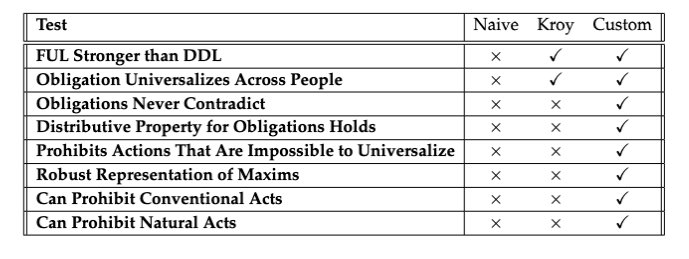
\includegraphics[scale=0.6]{goalstable.png}
\caption{Table showing which tests each implementation passes. ``Naive'' indicates raw DDL, 
``Kroy'' is my implementation of Moshe Kroy's formalization of the FUL, and ``Custom'' is my novel implementation.} \label{table}
\end{figure}
%
\begin{isamarkuptext}%
\noindent \textbf{FUL Stronger than DDL} The FUL should not hold in raw DDL, which I use a control group. 
If the FUL holds in the base logic, then adding it as an axiom doesn't make the logic any stronger, 
which is troubling because the base logic does not come equipped with the categorical imperative. DDL
defines basic properties of obligation, such as ought implies can, but contains no axioms that represent
the Formula of Universal Law. Therefore, if a formalization of the FUL holds in the 
base logic, then it is too weak to actually represent the FUL. Both Kroy's formalization
and my implementation do not hold in the base logic, and thus represent progress over the control group.
To test this property, I used Nitpick to find a countermodel in which my version of the FUL does not hold. 
I performed this test before adding the FUL as an axiom, since after adding it no countermodel will
be possible.%
\end{isamarkuptext}\isamarkuptrue%
%
\begin{isamarkuptext}%
\medskip
\noindent \textbf{Obligation Universalizes Across People} The obligations prescribed by the Formula of Universal Law
should generalize across people. In other words, if a maxim is obligated for one person, then it is obligated
for all other people because maxims are not person-specific. Velleman argues that, because 
reason is accessible to everyone identically, obligations apply to all people equally \citep[25]{velleman}. 
When Kant describes the categorical imperative as the objective principle of the will, he is referring 
to the fact that, as opposed to a subjective principle, the categorical imperative applies to all 
rational agents equally \citep[16]{groundwork}. At its core, the FUL best handles, ``the temptation 
to make oneself an exception: selfishness, meanness, advantagetaking, and disregard for the rights 
of others'' \citep[30]{KorsgaardFUL}. Kroy makes this property the center of his
formalization, which essentially says that if an act is permissible for someone, it is permissible for 
everyone.\footnote{Formally, $P\{A(s)\} \longrightarrow \forall p. P\{A(p)\}$.} Kroy's formalization and 
my formalization satisfy this property, but raw DDL does not. Below I run
this test for my formalization.%
\end{isamarkuptext}\isamarkuptrue%
\isacommand{lemma}\isamarkupfalse%
\ wrong{\isacharunderscore}if{\isacharunderscore}wrong{\isacharunderscore}for{\isacharunderscore}someone{\isacharcolon}\isanewline
\ \ \isakeyword{shows}\ {\isachardoublequoteopen}{\isasymforall}w{\isachardot}\ {\isasymforall}c{\isacharcolon}{\isacharcolon}t{\isachardot}\ {\isasymforall}g{\isacharcolon}{\isacharcolon}t{\isachardot}\ {\isasymforall}a{\isachardot}\ {\isasymexists}s{\isacharcolon}{\isacharcolon}s{\isachardot}\ O{\isacharbraceleft}\isactrlbold {\isasymnot}\ {\isacharparenleft}W\ {\isacharparenleft}c{\isacharcomma}\ a{\isacharcomma}\ g{\isacharparenright}\ s{\isacharparenright}\ {\isacharbar}\ c{\isacharbraceright}\ w\ {\isasymlongrightarrow}\ {\isacharparenleft}{\isasymforall}p{\isachardot}\ \ O{\isacharbraceleft}\isactrlbold {\isasymnot}\ {\isacharparenleft}W\ {\isacharparenleft}c{\isacharcomma}\ a{\isacharcomma}\ g{\isacharparenright}\ p{\isacharparenright}\ {\isacharbar}\ c{\isacharbraceright}\ w{\isacharparenright}\ {\isachardoublequoteclose}\isanewline
%
\isadelimproof
\ \ %
\endisadelimproof
%
\isatagproof
\isacommand{by}\isamarkupfalse%
\ blast\isanewline
%
\isamarkupcmt{I represent my tests as 
lemmas that I expect Isabelle to either prove or refute. The statement following the keyword \texttt{shows}
is the sentence of the lemma, and the proof follows the \texttt{by} keyword%
}\isanewline
%
\isamarkupcmt{This lemma shows that if a maxim $(c, a, g)$ is wrong for subject $s$ at a world, then it is wrong
for all people at that world. Isabelle automatically completed this proof using the \texttt{blast} method, 
which implements a generic tableau prover, a proof method that operates on lists of formulae using 
rules for conjunction, disjunction, universal quantification, and existential quantification \citep{blast}.%
}%
\endisatagproof
{\isafoldproof}%
%
\isadelimproof
\isanewline
%
\endisadelimproof
\isanewline
\isacommand{lemma}\isamarkupfalse%
\ right{\isacharunderscore}if{\isacharunderscore}right{\isacharunderscore}for{\isacharunderscore}someone{\isacharcolon}\isanewline
\ \ \isakeyword{shows}\ {\isachardoublequoteopen}{\isasymforall}w{\isachardot}\ {\isasymforall}c{\isacharcolon}{\isacharcolon}t{\isachardot}\ {\isasymforall}g{\isacharcolon}{\isacharcolon}t{\isachardot}\ {\isasymforall}a{\isachardot}\ {\isasymexists}s{\isacharcolon}{\isacharcolon}s{\isachardot}\ O{\isacharbraceleft}W\ {\isacharparenleft}c{\isacharcomma}\ a{\isacharcomma}\ g{\isacharparenright}\ s\ {\isacharbar}\ c{\isacharbraceright}\ w\ {\isasymlongrightarrow}\ {\isacharparenleft}{\isasymforall}p{\isachardot}\ \ O{\isacharbraceleft}W\ {\isacharparenleft}c{\isacharcomma}\ a{\isacharcomma}\ g{\isacharparenright}\ p\ {\isacharbar}\ c{\isacharbraceright}\ w{\isacharparenright}\ {\isachardoublequoteclose}\isanewline
%
\isadelimproof
\ \ %
\endisadelimproof
%
\isatagproof
\isacommand{by}\isamarkupfalse%
\ blast\isanewline
%
\isamarkupcmt{This lemma shows that if a maxim $(c, a, g)$ is right for subject $s$ at a world, then it is right
for all people at that world. The proof similarly proceeds using \texttt{blast}.%
}%
\endisatagproof
{\isafoldproof}%
%
\isadelimproof
%
\endisadelimproof
%
\begin{isamarkuptext}%
\noindent \textbf{Obligations Never Contradict} Contradictory obligations
make obeying the prescriptions of an ethical theory impossible.
Kant subscribes to the general, popular view that morality is supposed to guide action, so ought implies 
can.\footnote{Kohl points out that this principle is referred to as 
Kant's dictum or Kant's law in the literature \citep[footnote 1]{kohl}.} Kohl reconstructs Kant's argument for this principle as 
follows: if the will cannot comply with the moral law, then the moral law has no prescriptive authority 
for the will \citep[703-4]{kohl}. This defeats the purpose of Kant's theory, which is to develop an unconditional, categorical imperative 
for rational agents. Ought implies can requires that obligations never contradict each other, because an agent 
can't perform contradictory actions. Therefore, any ethical theory that respects ought implies can, 
and Kantian ethics in particular, must not result in conflicting obligations. 
Kant only briefly discusses contradictory obligations in \emph{Metaphysics of Morals}, where he argues that 
conflicting moral obligations are impossible under his theory \citep[V224]{metaphysicsintro}. Particularly, the categorical imperative generates 
``strict negative laws of omission,'' which cannot conflict by definition \citep[45]{timmerman}.\footnote{The 
kinds of obligations generated by the FUL are called ``perfect duties'' which arise from ``contradictions 
in conception,'' or maxims that we cannot even concieve of universalizing. These duties are always negative 
and thus never conflict. Kant also presents ``imperfect duties,'' generated from ``contradictions in will,''
or maxims that we can concieve of universalizing but would never want to. These duties tend to be broader, 
such as ``improve oneself" or "help others," and are secondary to perfect duties. My project only analyzes 
perfect duties, as these are always stronger than imperfect duties.} Both raw DDL and 
Kroy's formalization allow contradictory obligations, but I explicitly add an axiom to my formalization
that prohibits contradictory obligations.%
\end{isamarkuptext}\isamarkuptrue%
\isacommand{lemma}\isamarkupfalse%
\ conflicting{\isacharunderscore}obligations{\isacharcolon}\isanewline
\ \ \isakeyword{shows}\ {\isachardoublequoteopen}{\isasymnot}\ {\isacharparenleft}O{\isacharbraceleft}W\ {\isacharparenleft}c{\isacharcomma}\ a{\isacharcomma}\ g{\isacharparenright}\ s{\isacharbar}c{\isacharbraceright}\ \isactrlbold {\isasymand}\ O{\isacharbraceleft}\isactrlbold {\isasymnot}{\isacharparenleft}W\ {\isacharparenleft}c{\isacharcomma}\ a{\isacharcomma}\ g{\isacharparenright}\ s{\isacharparenright}{\isacharbar}\ c{\isacharbraceright}{\isacharparenright}\ w{\isachardoublequoteclose}\isanewline
%
\isadelimproof
\ \ %
\endisadelimproof
%
\isatagproof
\isacommand{using}\isamarkupfalse%
\ no{\isacharunderscore}contradictions\ \isacommand{by}\isamarkupfalse%
\ blast\isanewline
%
\isamarkupcmt{This test passes immediately by the new axiom that prohibits contradictory obligations.%
}%
\endisatagproof
{\isafoldproof}%
%
\isadelimproof
\isanewline
%
\endisadelimproof
\isanewline
\isacommand{lemma}\isamarkupfalse%
\ implied{\isacharunderscore}contradiction{\isacharcolon}\isanewline
\ \ \isakeyword{assumes}\ {\isachardoublequoteopen}{\isacharparenleft}{\isacharparenleft}{\isacharparenleft}W\ {\isacharparenleft}c{\isadigit{1}}{\isacharcomma}\ a{\isadigit{1}}{\isacharcomma}\ g{\isadigit{1}}{\isacharparenright}\ s{\isacharparenright}\ \isactrlbold {\isasymand}\ {\isacharparenleft}W\ {\isacharparenleft}c{\isadigit{2}}{\isacharcomma}\ a{\isadigit{2}}{\isacharcomma}\ g{\isadigit{2}}{\isacharparenright}\ s{\isacharparenright}{\isacharparenright}\ \isactrlbold {\isasymrightarrow}\ \isactrlbold {\isasymbottom}{\isacharparenright}\ w{\isachardoublequoteclose}\isanewline
\ \ \isakeyword{shows}\ {\isachardoublequoteopen}\isactrlbold {\isasymnot}\ {\isacharparenleft}O{\isacharbraceleft}W{\isacharparenleft}c{\isadigit{1}}{\isacharcomma}\ a{\isadigit{1}}{\isacharcomma}\ g{\isadigit{1}}{\isacharparenright}\ s{\isacharbar}c{\isacharbraceright}\ \isactrlbold {\isasymand}\ O{\isacharbraceleft}W{\isacharparenleft}c{\isadigit{2}}{\isacharcomma}\ a{\isadigit{2}}{\isacharcomma}\ g{\isadigit{2}}{\isacharparenright}\ s{\isacharbar}c{\isacharbraceright}{\isacharparenright}\ w{\isachardoublequoteclose}\isanewline
%
\isadelimproof
\ \ %
\endisadelimproof
%
\isatagproof
\isacommand{using}\isamarkupfalse%
\ assms\ no{\isacharunderscore}contradictions\ \isacommand{by}\isamarkupfalse%
\ blast\isanewline
%
\isamarkupcmt{This stronger property states that the combination of obligatory maxims can't
 imply a contradiction and should hold for the same reasons that contradictory obligations aren't
allowed. The added axiom also makes this test pass.%
}%
\endisatagproof
{\isafoldproof}%
%
\isadelimproof
%
\endisadelimproof
%
\begin{isamarkuptext}%
Contradictory obligations are closely related to two other properties. First is the idea that obligation implies permissibility, or 
that obligation is a stronger property than permissibility. If there are no contradictory obligations, 
then this property holds because actions are either permissible or prohibited and obligation contradicts
prohibition. In a system with contradictory obligations, this property fails because there is some
maxim that is obligated but also prohibited and therefore not permisible. The simple proof below 
shows that this property is incompatible with contradictory obligations.

\medskip%
\end{isamarkuptext}\isamarkuptrue%
\isacommand{lemma}\isamarkupfalse%
\ {\isachardoublequoteopen}{\isasymforall}w{\isachardot}\ {\isasymexists}A{\isachardot}\ {\isacharparenleft}{\isacharparenleft}{\isacharparenleft}O\ {\isacharbraceleft}A{\isacharbraceright}\ \isactrlbold {\isasymand}\ O\ {\isacharbraceleft}\isactrlbold {\isasymnot}\ A{\isacharbraceright}{\isacharparenright}w{\isacharparenright}{\isacharparenright}\ {\isasymequiv}\ {\isacharparenleft}{\isasymexists}B{\isachardot}\ {\isacharparenleft}\isactrlbold {\isasymnot}\ {\isacharparenleft}O\ {\isacharbraceleft}B{\isacharbraceright}\ \isactrlbold {\isasymrightarrow}\ \isactrlbold {\isasymnot}\ O\ {\isacharbraceleft}\isactrlbold {\isasymnot}B{\isacharbraceright}{\isacharparenright}{\isacharparenright}\ w{\isacharparenright}{\isachardoublequoteclose}\isanewline
%
\isadelimproof
\ \ %
\endisadelimproof
%
\isatagproof
\isacommand{by}\isamarkupfalse%
\ simp\isanewline
%
\isamarkupcmt{This lemma shows that if there is some maxim $A$ such that $A$ and $\neg A$ are both obligatory (which
is the formal statement of contradictory obligations), then obligation does not always imply permissibility.%
}\isanewline
%
\isamarkupcmt{\texttt{simp} is the simplification tactic, which unfolds definitions to complete a proof.%
}%
\endisatagproof
{\isafoldproof}%
%
\isadelimproof
%
\endisadelimproof
%
\begin{isamarkuptext}%
\noindent \textbf{Distributive Property for Obligations Holds} Another property related to contradictory obligations is the distributive property for the obligation
operator.\footnote{Formally, $O\{A\} \wedge O\{B\} \longleftrightarrow O\{A \wedge B\}$.} This is 
another property that we expect to hold. The rough English translation of  $O \{ A \wedge B \} $ is ``you are obligated to 
do both A and B''. The rough English translation of $O\{A\} \wedge O\{B\}$ is ``you are obligated to do A 
and you are obligated to do B.'' We think those English sentences mean the same thing, and they should mean 
the same thing in logic as well. Moreover, if that (rather intuitive) property holds, then contradictory
obligations are impossible, as shown in the below proof.%
\end{isamarkuptext}\isamarkuptrue%
\isacommand{lemma}\isamarkupfalse%
\ distributive{\isacharunderscore}implies{\isacharunderscore}no{\isacharunderscore}contradictions{\isacharcolon}\ \isanewline
\ \ \isakeyword{assumes}\ {\isachardoublequoteopen}{\isasymforall}A\ B{\isachardot}\ {\isasymTurnstile}\ {\isacharparenleft}{\isacharparenleft}O\ {\isacharbraceleft}A{\isacharbraceright}\ \isactrlbold {\isasymand}\ O\ {\isacharbraceleft}B{\isacharbraceright}{\isacharparenright}\ \isactrlbold {\isasymequiv}\ O\ {\isacharbraceleft}A\ \isactrlbold {\isasymand}\ B{\isacharbraceright}{\isacharparenright}{\isachardoublequoteclose}\isanewline
\ \ \isakeyword{shows}\ {\isachardoublequoteopen}{\isasymforall}A{\isachardot}\ {\isasymTurnstile}{\isacharparenleft}\ \isactrlbold {\isasymnot}{\isacharparenleft}O\ {\isacharbraceleft}A{\isacharbraceright}\ \isactrlbold {\isasymand}\ O\ {\isacharbraceleft}\isactrlbold {\isasymnot}\ A{\isacharbraceright}{\isacharparenright}{\isacharparenright}\ {\isachardoublequoteclose}\isanewline
%
\isadelimproof
\ \ %
\endisadelimproof
%
\isatagproof
\isacommand{using}\isamarkupfalse%
\ O{\isacharunderscore}diamond\ assms\ \isacommand{by}\isamarkupfalse%
\ blast\isanewline
%
\isamarkupcmt{The \texttt{assumes} keyword indicates assumptions used when proving a lemma. I use it here to 
represent metalogical implication. With the assumption, the lemma above reads, ``If the distributive
property holds in this logic, then obligations cannot contradict.''%
}%
\endisatagproof
{\isafoldproof}%
%
\isadelimproof
%
\endisadelimproof
%
\begin{isamarkuptext}%
Again, this test fails for raw DDL and for Kroy's formalization, but
passes for my interpretation because I require that obligations don't contradict as an axiom.%
\end{isamarkuptext}\isamarkuptrue%
\isacommand{lemma}\isamarkupfalse%
\ distribution{\isacharcolon}\isanewline
\ \ \isakeyword{assumes}\ {\isachardoublequoteopen}{\isasymTurnstile}\ {\isacharparenleft}O\ {\isacharbraceleft}A{\isacharbraceright}\ \isactrlbold {\isasymand}\ O\ {\isacharbraceleft}B{\isacharbraceright}{\isacharparenright}{\isachardoublequoteclose}\isanewline
\ \ \isakeyword{shows}\ {\isachardoublequoteopen}{\isasymTurnstile}\ O\ {\isacharbraceleft}A\ \isactrlbold {\isasymand}\ B{\isacharbraceright}{\isachardoublequoteclose}\isanewline
%
\isadelimproof
\ \ %
\endisadelimproof
%
\isatagproof
\isacommand{using}\isamarkupfalse%
\ assms\ no{\isacharunderscore}contradictions\ \isacommand{by}\isamarkupfalse%
\ fastforce\isanewline
%
\isamarkupcmt{The proof proceeds almost immediately using the new axiom.%
}%
\endisatagproof
{\isafoldproof}%
%
\isadelimproof
%
\endisadelimproof
%
\begin{isamarkuptext}%
\medskip 

\noindent \textbf{Prohibits Actions That Are Impossible to Universalize} Recall that 
the logical contradiction interpretation of the Formula of Universal Law prohibits lying because in a world 
where everyone simultaneously lies, lying is impossible. In other words, not everyone can simultaneously
lie because the institution of lying and believing would break down. In Section \ref{praccon}, 
I recreated Korsgaard's argument for why the logical contradiction interpretation is weaker than what the
Formula of Universal Law should actually require. Therefore, any implementation of the FUL should be 
able to show that the actions prohibited by the logical contradiction interpretation are prohibited, 
because the set of actions prohibited by the practical contradiction interpretation is a superset of these.
The FUL should show that actions that cannot possibly be universalized are prohibited, because those acts cannot be willed in 
a world where they are universalized. This property fails to hold in both raw DDL
and Kroy's formalization, but holds for my formalization. Showing that this property holds
for my formalization required significant logical work and the full code is presented in Appendix \ref{weirdtests}.%
\end{isamarkuptext}\isamarkuptrue%
%
\begin{isamarkuptext}%
\noindent \textbf{Robust Representation of Maxims} Kant does not evaluate the correctness of acts, but rather of maxims. Therefore, any 
faithful formalization of the categorical imperative must evaluate maxims, not acts. This requires 
representing a maxim and making it the input to the obligation operator, which only my implementation 
does. Because my implementation includes the notion of a maxim, it is able to perform sophisticated 
reasoning as demonstrated in Sections \ref{joking} and \ref{murderer}. Staying faithful to the philosophical 
literature enables my system to make more reliable judgements.

\medskip%
\end{isamarkuptext}\isamarkuptrue%
%
\begin{isamarkuptext}%
\noindent \textbf{Can Prohibit Conventional and Natural Acts} When arguing for the practical contradiction interpretation,
Korsgaard makes a distinction between conventional and natural acts \citep{KorsgaardFUL}. 
A conventional act relies on a convention, like the 
convention that a promise is a commitment, whereas a natural act is possible simply because of the laws 
of the natural world. Conventional acts exist within a practice, which is ``comprised of certain rules, 
and its existence (where it is not embodied in an institution with sanctions) consists in the general 
acknowledgement and following of those rules'' \cite[10]{KorsgaardFUL}. Promising is a conventional act 
because it exists as a practice. Murder, on the other hand, is an example of a natural act because 
its existence only depends on the laws of nature\cite[11]{KorsgaardFUL}.

It is easier to show the wrongness of conventional acts because there are worlds
in which these acts are impossible; namely, worlds in which the convention does not exist. For example, 
the common argument against falsely promising is that if everyone were to falsely promise, the convention 
of promising would fall apart because people wouldn't believe each other, so falsely promising is prohibited. 
It is more difficult to show the wrongness of a natural act, like murder or violence. These acts can 
never be logically impossible; even if everyone murders or acts violently, murder and violence will 
still be possible, so it is difficult to show that they violate the FUL. 

Both raw DDL and Kroy's interpretation fail to show the wrongness of conventional or natural acts. 
My system shows the wrongness of both natural and conventional acts because it is faithful to Korsgaard's 
practical contradiction interpretation of the FUL, which is the canonical interpretation of the 
FUL \citep{ebelsduggan, KorsgaardFUL}. I run this test in Chapter \ref{applications}, where I
use my system to reason about two ethical dilemmas, one which involves conventional acts and the other which
involves natural acts. I present an additional example demonstrating that my implementation passes
this test in Appendix \ref{weirdtests}.%
\end{isamarkuptext}\isamarkuptrue%
%
\isadelimproof
%
\endisadelimproof
%
\isatagproof
%
\endisatagproof
{\isafoldproof}%
%
\isadelimproof
%
\endisadelimproof
%
\isadelimtheory
%
\endisadelimtheory
%
\isatagtheory
%
\endisatagtheory
{\isafoldtheory}%
%
\isadelimtheory
%
\endisadelimtheory
%
\end{isabellebody}%
\endinput
%:%file=~/Desktop/cs91r/paper/thesis_3_implementation.thy%:%
%:%24=6%:%
%:%36=8%:%
%:%37=9%:%
%:%38=10%:%
%:%39=11%:%
%:%40=12%:%
%:%41=13%:%
%:%42=14%:%
%:%43=15%:%
%:%52=17%:%
%:%64=19%:%
%:%65=20%:%
%:%66=21%:%
%:%67=22%:%
%:%76=24%:%
%:%88=26%:%
%:%89=27%:%
%:%90=28%:%
%:%91=29%:%
%:%92=30%:%
%:%94=32%:%
%:%95=32%:%
%:%96=32%:%
%:%99=34%:%
%:%100=35%:%
%:%101=36%:%
%:%102=37%:%
%:%103=38%:%
%:%104=39%:%
%:%105=40%:%
%:%106=41%:%
%:%107=42%:%
%:%108=43%:%
%:%109=44%:%
%:%110=45%:%
%:%111=46%:%
%:%112=47%:%
%:%113=48%:%
%:%114=49%:%
%:%116=51%:%
%:%117=51%:%
%:%119=52%:%
%:%120=53%:%
%:%121=54%:%
%:%122=55%:%
%:%123=56%:%
%:%124=57%:%
%:%125=58%:%
%:%126=59%:%
%:%134=61%:%
%:%146=63%:%
%:%147=64%:%
%:%148=65%:%
%:%149=66%:%
%:%150=67%:%
%:%151=68%:%
%:%152=69%:%
%:%153=70%:%
%:%154=71%:%
%:%155=72%:%
%:%156=73%:%
%:%157=74%:%
%:%158=75%:%
%:%159=76%:%
%:%160=77%:%
%:%161=78%:%
%:%162=79%:%
%:%163=80%:%
%:%164=81%:%
%:%165=82%:%
%:%166=83%:%
%:%167=84%:%
%:%168=85%:%
%:%169=86%:%
%:%170=87%:%
%:%171=88%:%
%:%172=89%:%
%:%174=92%:%
%:%175=92%:%
%:%177=93%:%
%:%178=94%:%
%:%179=95%:%
%:%180=96%:%
%:%181=97%:%
%:%182=98%:%
%:%183=99%:%
%:%184=100%:%
%:%187=102%:%
%:%188=103%:%
%:%189=104%:%
%:%190=105%:%
%:%191=106%:%
%:%192=107%:%
%:%193=108%:%
%:%194=109%:%
%:%195=110%:%
%:%196=111%:%
%:%197=112%:%
%:%198=113%:%
%:%199=114%:%
%:%200=115%:%
%:%201=116%:%
%:%202=117%:%
%:%203=118%:%
%:%204=119%:%
%:%205=120%:%
%:%206=121%:%
%:%207=122%:%
%:%208=123%:%
%:%209=124%:%
%:%210=125%:%
%:%211=126%:%
%:%212=127%:%
%:%213=128%:%
%:%214=129%:%
%:%215=130%:%
%:%216=131%:%
%:%217=132%:%
%:%218=133%:%
%:%219=134%:%
%:%220=135%:%
%:%221=136%:%
%:%222=137%:%
%:%223=138%:%
%:%224=139%:%
%:%225=140%:%
%:%226=141%:%
%:%227=142%:%
%:%228=143%:%
%:%230=145%:%
%:%231=145%:%
%:%232=146%:%
%:%234=147%:%
%:%235=148%:%
%:%236=149%:%
%:%237=150%:%
%:%245=152%:%
%:%257=154%:%
%:%258=155%:%
%:%259=156%:%
%:%260=157%:%
%:%261=158%:%
%:%262=159%:%
%:%263=160%:%
%:%264=161%:%
%:%265=162%:%
%:%266=163%:%
%:%267=164%:%
%:%268=165%:%
%:%269=166%:%
%:%270=167%:%
%:%271=168%:%
%:%272=169%:%
%:%273=170%:%
%:%274=171%:%
%:%275=172%:%
%:%276=173%:%
%:%277=174%:%
%:%278=175%:%
%:%279=176%:%
%:%280=177%:%
%:%281=178%:%
%:%282=179%:%
%:%283=180%:%
%:%284=181%:%
%:%285=182%:%
%:%286=183%:%
%:%287=184%:%
%:%288=185%:%
%:%289=186%:%
%:%290=187%:%
%:%291=188%:%
%:%292=189%:%
%:%293=190%:%
%:%294=191%:%
%:%295=192%:%
%:%296=193%:%
%:%297=194%:%
%:%298=195%:%
%:%299=196%:%
%:%300=197%:%
%:%301=198%:%
%:%302=199%:%
%:%303=200%:%
%:%304=201%:%
%:%305=202%:%
%:%306=203%:%
%:%307=204%:%
%:%308=205%:%
%:%310=208%:%
%:%311=208%:%
%:%312=209%:%
%:%314=210%:%
%:%315=211%:%
%:%318=213%:%
%:%319=214%:%
%:%320=215%:%
%:%321=216%:%
%:%322=217%:%
%:%323=218%:%
%:%324=219%:%
%:%325=220%:%
%:%326=221%:%
%:%327=222%:%
%:%328=223%:%
%:%329=224%:%
%:%330=225%:%
%:%331=226%:%
%:%332=227%:%
%:%333=228%:%
%:%334=229%:%
%:%335=230%:%
%:%337=233%:%
%:%338=233%:%
%:%339=234%:%
%:%341=235%:%
%:%342=236%:%
%:%345=240%:%
%:%346=241%:%
%:%347=242%:%
%:%348=243%:%
%:%349=244%:%
%:%350=245%:%
%:%351=246%:%
%:%352=247%:%
%:%353=248%:%
%:%354=249%:%
%:%355=250%:%
%:%357=252%:%
%:%358=252%:%
%:%359=253%:%
%:%361=254%:%
%:%364=256%:%
%:%365=257%:%
%:%366=258%:%
%:%367=259%:%
%:%368=260%:%
%:%369=261%:%
%:%370=262%:%
%:%371=263%:%
%:%372=264%:%
%:%373=265%:%
%:%374=266%:%
%:%375=267%:%
%:%376=268%:%
%:%377=269%:%
%:%378=270%:%
%:%379=271%:%
%:%380=272%:%
%:%381=273%:%
%:%382=274%:%
%:%383=275%:%
%:%384=276%:%
%:%385=277%:%
%:%386=278%:%
%:%387=279%:%
%:%388=280%:%
%:%389=281%:%
%:%390=282%:%
%:%391=283%:%
%:%392=284%:%
%:%393=285%:%
%:%394=286%:%
%:%395=287%:%
%:%396=288%:%
%:%398=290%:%
%:%399=290%:%
%:%400=291%:%
%:%402=292%:%
%:%403=293%:%
%:%404=293%:%
%:%405=294%:%
%:%406=294%:%
%:%407=295%:%
%:%409=296%:%
%:%410=297%:%
%:%413=298%:%
%:%414=299%:%
%:%415=300%:%
%:%416=301%:%
%:%418=303%:%
%:%419=303%:%
%:%420=304%:%
%:%422=305%:%
%:%423=306%:%
%:%424=306%:%
%:%425=307%:%
%:%426=307%:%
%:%428=308%:%
%:%429=309%:%
%:%430=310%:%
%:%438=312%:%
%:%450=314%:%
%:%451=315%:%
%:%452=316%:%
%:%453=317%:%
%:%454=318%:%
%:%455=319%:%
%:%456=320%:%
%:%457=321%:%
%:%459=324%:%
%:%460=324%:%
%:%462=325%:%
%:%463=326%:%
%:%464=327%:%
%:%465=328%:%
%:%468=330%:%
%:%469=331%:%
%:%471=333%:%
%:%472=333%:%
%:%474=333%:%
%:%478=333%:%
%:%479=333%:%
%:%480=334%:%
%:%481=334%:%
%:%482=334%:%
%:%491=336%:%
%:%492=337%:%
%:%493=338%:%
%:%494=339%:%
%:%495=340%:%
%:%496=341%:%
%:%497=342%:%
%:%498=343%:%
%:%499=344%:%
%:%500=345%:%
%:%501=346%:%
%:%502=347%:%
%:%503=348%:%
%:%504=349%:%
%:%505=350%:%
%:%506=351%:%
%:%507=352%:%
%:%508=353%:%
%:%509=354%:%
%:%510=355%:%
%:%511=356%:%
%:%512=357%:%
%:%513=358%:%
%:%515=360%:%
%:%516=360%:%
%:%517=361%:%
%:%519=362%:%
%:%520=363%:%
%:%523=365%:%
%:%525=367%:%
%:%526=367%:%
%:%527=368%:%
%:%529=369%:%
%:%530=370%:%
%:%531=370%:%
%:%532=371%:%
%:%533=372%:%
%:%534=372%:%
%:%535=373%:%
%:%536=373%:%
%:%538=373%:%
%:%542=373%:%
%:%543=373%:%
%:%545=374%:%
%:%546=375%:%
%:%547=376%:%
%:%548=377%:%
%:%549=378%:%
%:%550=379%:%
%:%551=380%:%
%:%561=382%:%
%:%562=383%:%
%:%563=384%:%
%:%564=385%:%
%:%565=386%:%
%:%566=387%:%
%:%567=388%:%
%:%568=389%:%
%:%569=390%:%
%:%570=391%:%
%:%571=392%:%
%:%572=393%:%
%:%573=394%:%
%:%574=395%:%
%:%575=396%:%
%:%576=397%:%
%:%577=398%:%
%:%578=399%:%
%:%579=400%:%
%:%580=401%:%
%:%582=403%:%
%:%583=403%:%
%:%585=405%:%
%:%586=406%:%
%:%587=407%:%
%:%588=408%:%
%:%589=409%:%
%:%598=411%:%
%:%610=413%:%
%:%611=414%:%
%:%612=415%:%
%:%613=416%:%
%:%614=417%:%
%:%615=418%:%
%:%616=419%:%
%:%617=420%:%
%:%618=421%:%
%:%619=422%:%
%:%620=423%:%
%:%621=424%:%
%:%622=425%:%
%:%623=426%:%
%:%624=427%:%
%:%625=428%:%
%:%626=429%:%
%:%627=430%:%
%:%628=431%:%
%:%629=432%:%
%:%630=433%:%
%:%631=434%:%
%:%632=435%:%
%:%633=436%:%
%:%634=437%:%
%:%637=441%:%
%:%638=442%:%
%:%639=443%:%
%:%640=444%:%
%:%641=445%:%
%:%642=446%:%
%:%645=448%:%
%:%646=449%:%
%:%647=450%:%
%:%648=451%:%
%:%649=452%:%
%:%650=453%:%
%:%651=454%:%
%:%652=455%:%
%:%653=456%:%
%:%654=457%:%
%:%658=459%:%
%:%659=460%:%
%:%660=461%:%
%:%661=462%:%
%:%662=463%:%
%:%663=464%:%
%:%664=465%:%
%:%665=466%:%
%:%666=467%:%
%:%667=468%:%
%:%668=469%:%
%:%669=470%:%
%:%670=471%:%
%:%671=472%:%
%:%673=474%:%
%:%674=474%:%
%:%675=475%:%
%:%678=476%:%
%:%682=476%:%
%:%683=476%:%
%:%685=477%:%
%:%686=478%:%
%:%687=479%:%
%:%688=479%:%
%:%690=480%:%
%:%691=481%:%
%:%692=482%:%
%:%693=483%:%
%:%699=483%:%
%:%702=484%:%
%:%703=485%:%
%:%704=485%:%
%:%705=486%:%
%:%708=487%:%
%:%712=487%:%
%:%713=487%:%
%:%715=488%:%
%:%716=489%:%
%:%726=491%:%
%:%727=492%:%
%:%728=493%:%
%:%729=494%:%
%:%730=495%:%
%:%731=496%:%
%:%732=497%:%
%:%733=498%:%
%:%734=499%:%
%:%735=500%:%
%:%736=501%:%
%:%737=502%:%
%:%738=503%:%
%:%739=504%:%
%:%740=505%:%
%:%741=506%:%
%:%742=507%:%
%:%743=508%:%
%:%744=509%:%
%:%745=510%:%
%:%746=511%:%
%:%748=513%:%
%:%749=513%:%
%:%750=514%:%
%:%753=515%:%
%:%757=515%:%
%:%758=515%:%
%:%759=515%:%
%:%761=516%:%
%:%767=516%:%
%:%770=517%:%
%:%771=518%:%
%:%772=518%:%
%:%773=519%:%
%:%774=520%:%
%:%777=521%:%
%:%781=521%:%
%:%782=521%:%
%:%783=521%:%
%:%785=522%:%
%:%786=523%:%
%:%787=524%:%
%:%797=526%:%
%:%798=527%:%
%:%799=528%:%
%:%800=529%:%
%:%801=530%:%
%:%802=531%:%
%:%803=532%:%
%:%804=533%:%
%:%806=536%:%
%:%807=536%:%
%:%810=537%:%
%:%814=537%:%
%:%815=537%:%
%:%817=538%:%
%:%818=539%:%
%:%819=539%:%
%:%821=540%:%
%:%831=542%:%
%:%832=543%:%
%:%833=544%:%
%:%834=545%:%
%:%835=546%:%
%:%836=547%:%
%:%837=548%:%
%:%839=550%:%
%:%840=550%:%
%:%841=551%:%
%:%842=552%:%
%:%845=553%:%
%:%849=553%:%
%:%850=553%:%
%:%851=553%:%
%:%853=554%:%
%:%854=555%:%
%:%855=556%:%
%:%865=558%:%
%:%866=559%:%
%:%868=561%:%
%:%869=561%:%
%:%870=562%:%
%:%871=563%:%
%:%874=564%:%
%:%878=564%:%
%:%879=564%:%
%:%880=564%:%
%:%882=565%:%
%:%892=567%:%
%:%893=568%:%
%:%894=569%:%
%:%895=570%:%
%:%896=571%:%
%:%897=572%:%
%:%898=573%:%
%:%899=574%:%
%:%900=575%:%
%:%901=576%:%
%:%902=577%:%
%:%903=578%:%
%:%904=579%:%
%:%905=580%:%
%:%909=584%:%
%:%910=585%:%
%:%911=586%:%
%:%912=587%:%
%:%913=588%:%
%:%914=589%:%
%:%915=590%:%
%:%916=591%:%
%:%920=594%:%
%:%921=595%:%
%:%922=596%:%
%:%923=597%:%
%:%924=598%:%
%:%925=599%:%
%:%926=600%:%
%:%927=601%:%
%:%928=602%:%
%:%929=603%:%
%:%930=604%:%
%:%931=605%:%
%:%932=606%:%
%:%933=607%:%
%:%934=608%:%
%:%935=609%:%
%:%936=610%:%
%:%937=611%:%
%:%938=612%:%
%:%939=613%:%
%:%940=614%:%
%:%941=615%:%
%:%942=616%:%
%:%943=617%:%
%:%944=618%:%